\documentclass[12pt]{article}

%------------------------------ tables
\usepackage{tabularx}
\usepackage{makecell}
 \usepackage{amsmath} 
%------------------------------ images
\usepackage{graphicx}
\usepackage{subcaption}

% footnotes
\setlength{\footnotesep}{0.6\baselineskip}

% Page layout
\usepackage[left=3cm,right=3cm,top=3cm,bottom=2cm]{geometry}
\setlength{\skip\footins}{2cm}

% Clickable toc and links styles
\usepackage{hyperref}
\hypersetup{
    colorlinks,
    citecolor=black,
    filecolor=black,
    linkcolor=black,
    urlcolor=black
}
\usepackage{url}

% Title spec
\usepackage{titlesec}
\titlespacing\section{0pt}{20pt}{10pt}
\titlespacing\subsection{0pt}{15pt}{10pt}
\titlespacing\subsubsection{0pt}{10pt}{5pt}

% Page numbering and head
\usepackage{lastpage}
\usepackage{fancyhdr}
\pagestyle{fancy}
\fancyhf{}
\setlength{\headheight}{15pt}


\begin{document}

\begin{titlepage}

\begin{center}
    { \textit{University of Bologna} }\\
    \vspace{5mm}
    { \textit{Social Network Analysis} }\\
\end{center}

\vspace{20mm}

\begin{center}
    {\LARGE{\bf Open Flights}}\\
\end{center}

\vspace{20mm}

\begin{center}
    {\LARGE{Analysis of OpenFilght's Airplane Routes}}\\
\end{center}

\vspace{30mm}

\begin{center}
    {\large{Brajucha Filippo 0001130613\\}}
    \vspace{5mm}
    {\large{Leonardo Dessì \\}}
    \vspace{5mm}
    {\large{Gianmarco Gabrielli  \\}}
    \vspace{5mm}
    {\large{Simone Rinaldi 0001140193\\}}
\end{center}

\vspace{40mm}

\end{titlepage}

\tableofcontents
\newpage
\section{Introduction}
The idea is to develop the analysis of the global network of airports and the air routes connecting them. \\
We founded a data source on the OpenFlights website (\hyperlink{https://openflights.org/}{link} and \hyperlink{https://github.com/jpatokal/openflights}{github-link}), which allow us to construct a graph representing this network. In the graph, the nodes represent the airports, while the edges represent the direct air routes between two different airports.\\ 
We weight the edges according to the number of flights or connections that exist between the various airports.\\
The main objective of the project is to identify the most relevant and strategic airports on a network level. We identified the airports that serve as major transit nodes and subsequently test the hypothesis that these airports are critical for the overall connectivity of the network.


\section{Problem and Motivation}
The air transportation network is one of the most complex and vital networks in modern society, enabling global connectivity and supporting economic growth. Despite its importance, this network is vulnerable to disruptions caused by natural disasters, geopolitical events, technical failures, and pandemics. These disruptions can have significant cascading effects, leading to delays, economic losses, and reduced global mobility. Therefore, understanding the structure of the airline network and identifying critical nodes (airports) is crucial for ensuring the stability and resilience of air travel.
\newline Air traffic represents a large-scale, real-world network with thousands of nodes (airports) and edges (air routes). Analyzing such a network presents an interesting challenge in terms of data processing, graph construction, and extracting meaningful insights. Moreover, air transportation is central to modern life, and improvements in understanding its network properties can contribute to better planning and management of air traffic systems.
\section{Dataset}

\subsection{Dataset Description: OpenFlights Air Route Network}
The dataset used for this project is derived from OpenFlights, a public resource for airline, airport, and route data. Specifically, the dataset is an \textbf{edgelist} format file that describes the global air transportation network. This dataset is particularly valuable for studying the structure and dynamics of global air travel.

\subsubsection{Source}
\begin{itemize}
    \item \textbf{URL}: \href{http://opsahl.co.uk/tnet/datasets/openflights.txt}{OpenFlights Dataset}
    \item \textbf{Provider}: The dataset is hosted on Tore Opsahl’s website, a notable source for network analysis datasets.
\end{itemize}

\subsubsection{Format and Structure}
The dataset is formatted as an edgelist, where each row represents a direct connection (route) between two airports. An edgelist is a common representation of a graph in network analysis, detailing the edges (connections) between nodes (airports). Each line contains the following key information:
\begin{enumerate}
    \item \textbf{Source Node (Airport)}: A numerical ID representing the airport where the route originates.
    \item \textbf{Destination Node (Airport)}: A numerical ID representing the airport where the route ends.
    \item \textbf{Weight (Number)}: An additional column representing the weight of the edge, often indicating frequency or capacity.
\end{enumerate}
Each node number is linked to a list (openflights\_airports.txt) where is possible to find all the info about the airport (for example the country, the city, the code, the coordinates etc).

\subsection{Key Characteristics}
\begin{itemize}
    \item \textbf{Nodes}: Airports, each uniquely identified by an ID.
    \item \textbf{Edges}: Direct flight routes connecting pairs of airports.
    \item \textbf{Network Type}:
    \begin{itemize}
        \item \textit{Directed}: Routes are directional, from source airport to destination airport.
        \item \textit{Weighted}: Depending on the data, edges might include weights for analyzing traffic intensity or other attributes.
    \end{itemize}
\end{itemize}

\section{Validity and Reliability}
Ensuring the validity and reliability of the model used in this study is essential for drawing
meaningful insights into the analysis of the various airports and routes.

\section{Measures and Results}
\subsection{Measures}
This dataset is ideal for exploring various network science topics, including:
\begin{itemize}
    \item \textbf{Degree Centrality}: Evaluate the relative importance of a node based on the number of direct connections it has. Airports with high degree centrality are those that serve as primary points of connectivity in the network by offering a larger number of direct flights to different destinations. This high connectivity makes them essential to the efficiency and accessibility of the overall air transportation network.
    \item \textbf{Betweenness Centrality}: Quantifies the extent to which a particular node serves as a bridge or intermediary in the network. In the context of air travel, it measures how frequently an airport lies on the shortest paths between other pairs of airports
    \item \textbf{Closeness Centrality}: It measures the average shortest path distance from a given airport to all other airports. Airports with high closeness centrality are those that can quickly reach, or be reached by, other airports in the network, making them strategically advantageous for minimizing travel time and improving accessibility.
    \item \textbf{Eigevector Centrality }: Measures how well-connected an airport is to others. An airport with high eigenvector centrality is one that not only has many connections but is also linked to other highly connected and influential hubs, amplifying its importance within the global air transportation network.
    \item \textbf{PageRank}: It evaluates the significance of an airport by considering not only the number of its connections but also the importance of the airports it is connected to. This metric highlights influential airports, even when many of their connections are to less prominent nodes.
    \item \textbf{Clustering Coefficient}: Quantifies how likely it is that an airport’s neighboring airports (i.e., those directly connected to it) are also connected to one another. It provides insights into the local interconnectedness of an airport's surrounding network.
    \item \textbf{K-core}: Identifies a subnetwork of airports that are highly interconnected, where each airport in the subnetwork has at least k connections to other airports in that subnetwork. The k-core helps to highlight core airports that are central to a more tightly knit cluster of airports within the broader network.
    \end{itemize}
\newpage
\subsection{Results}
\begin{minipage}{\textwidth}
    \subsubsection{Degree}
    \text{Here is represented a bar chart with the airports that have the highest degree score.}
    \centering
    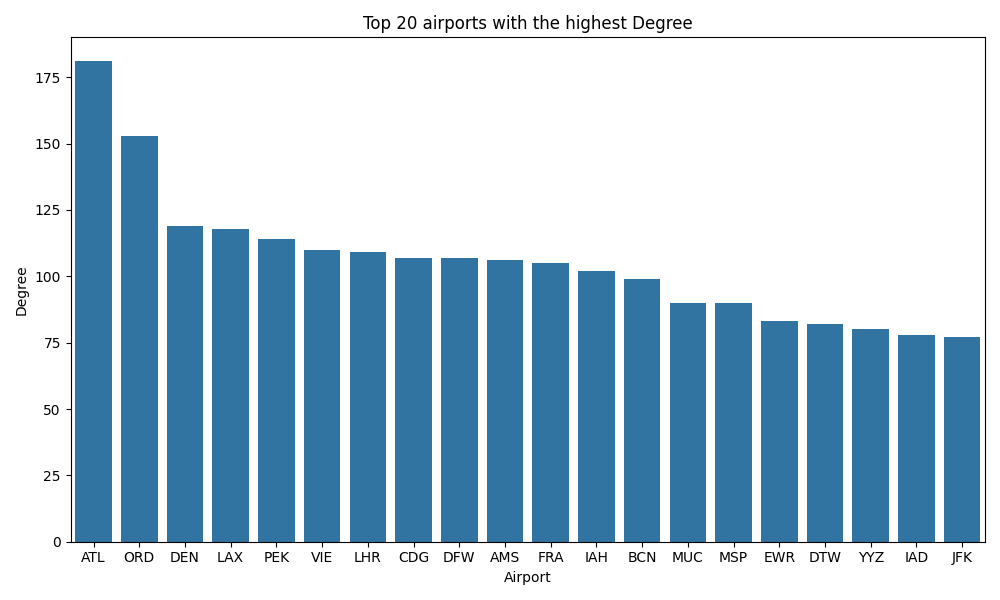
\includegraphics[width=1\linewidth]{img/degree.png}
\end{minipage}

\begin{minipage}{\textwidth}
    \subsubsection{Degree Centrality}
    {This chart shows the top 10 airports ranked by their degree centrality, which measures the number of direct connections an airport has with others. Hartsfield-Jackson Atlanta International Airport has the highest degree centrality, followed by Chicago O'Hare and Denver International Airports.}
    \centering
    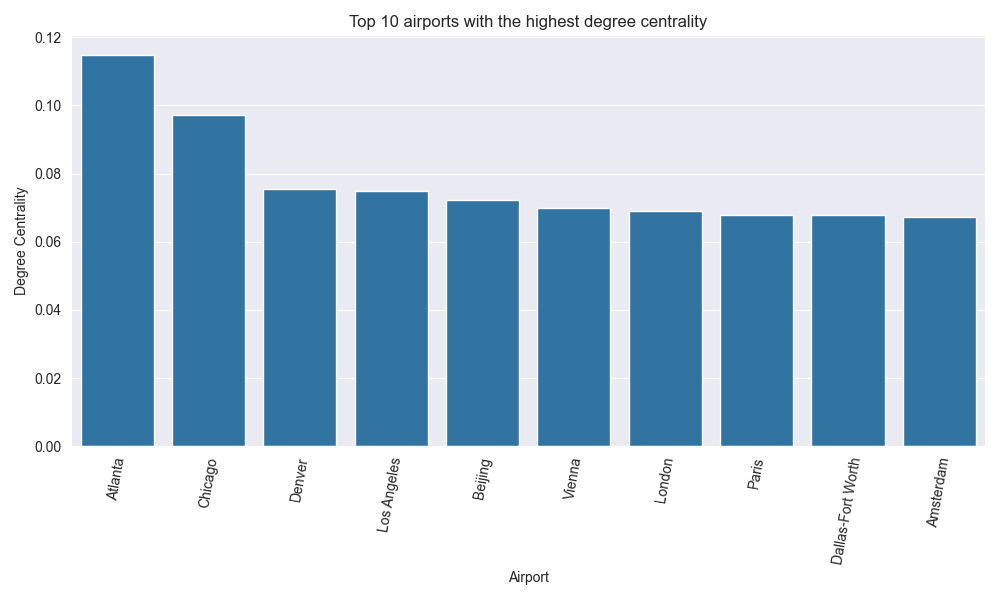
\includegraphics[width=1\linewidth]{img/degree_centrality.png}
\end{minipage}

\begin{minipage}{\textwidth}
    \subsubsection{Betweenness Centrality}
    {This bar chart shows the top 10 airports with the highest betweenness centrality. It how often an airport serves as a bridge along the shortest path between other airports, indicating its importance in connecting different parts of the air travel network.}
    \centering
    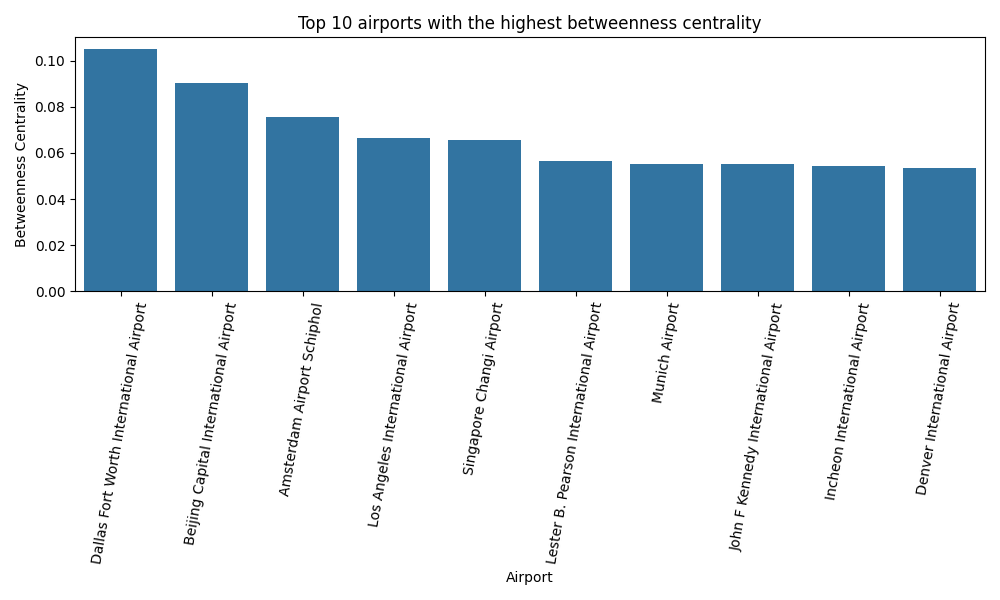
\includegraphics[width=1\linewidth]{img/betweenness_centrality.png}
\end{minipage}

\begin{minipage}{\textwidth}
    \subsubsection{Closeness Centrality}
    {In this chart are ranked the top 10 airports by closeness centrality, a measure of how well-connected an airport is within the network. These airports have similar levels of network connectivity. }
    \centering
    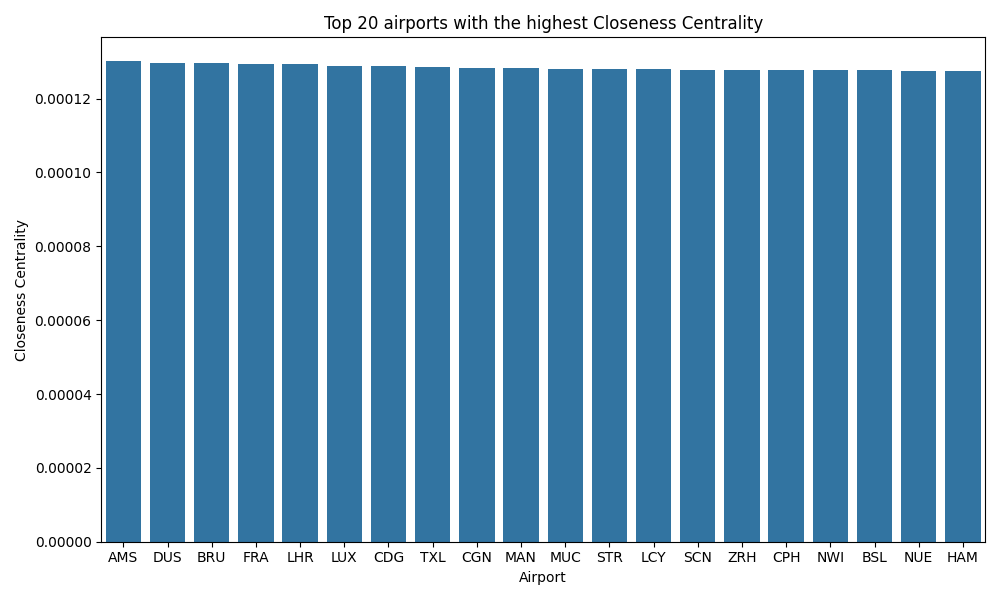
\includegraphics[width=1\linewidth]{img/closeness_centrality.png}
\end{minipage}

\begin{minipage}{\textwidth}
    \subsubsection{Clustering Coefficient}
   {This bar chart shows the top 10 airports by clustering coefficient, representing how well-connected an airport's neighboring airports are to each other. Chiang Mai International Airport leads with a coefficient of ~0.18, followed by Austin and Fort Smith at ~0.17 and ~0.15 respectively. The values decrease gradually to ~0.11 for Bujumbura International Airport. These airports serve as local hubs where connected airports also tend to connect with each other.}
    \centering
    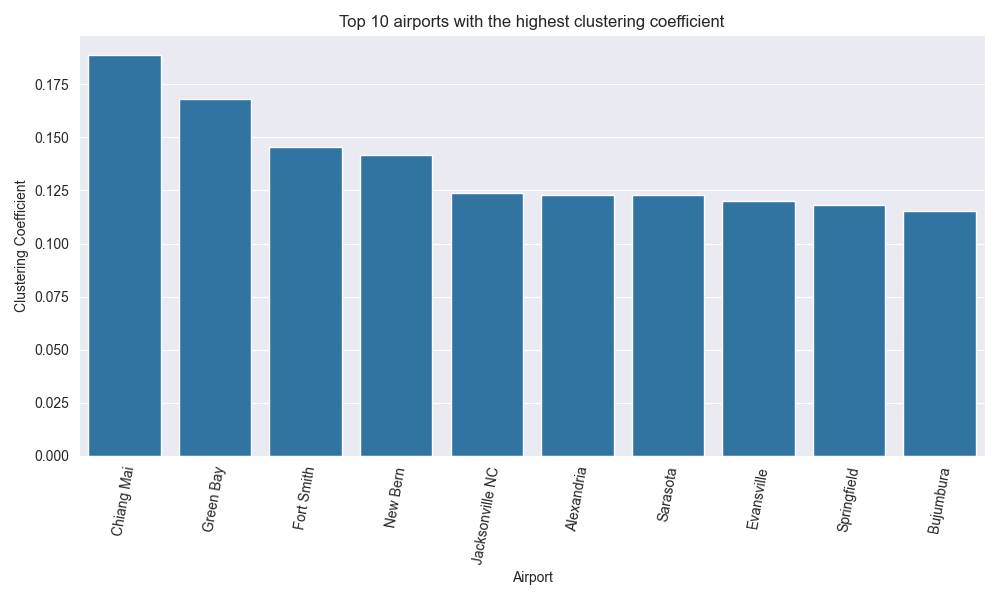
\includegraphics[width=1\linewidth]{img/clustering_coefficient.png}
\end{minipage}

\begin{minipage}{\textwidth}
    \subsubsection{K-core}
    {asadasdadasdadasdasdadasdas}
    \centering
    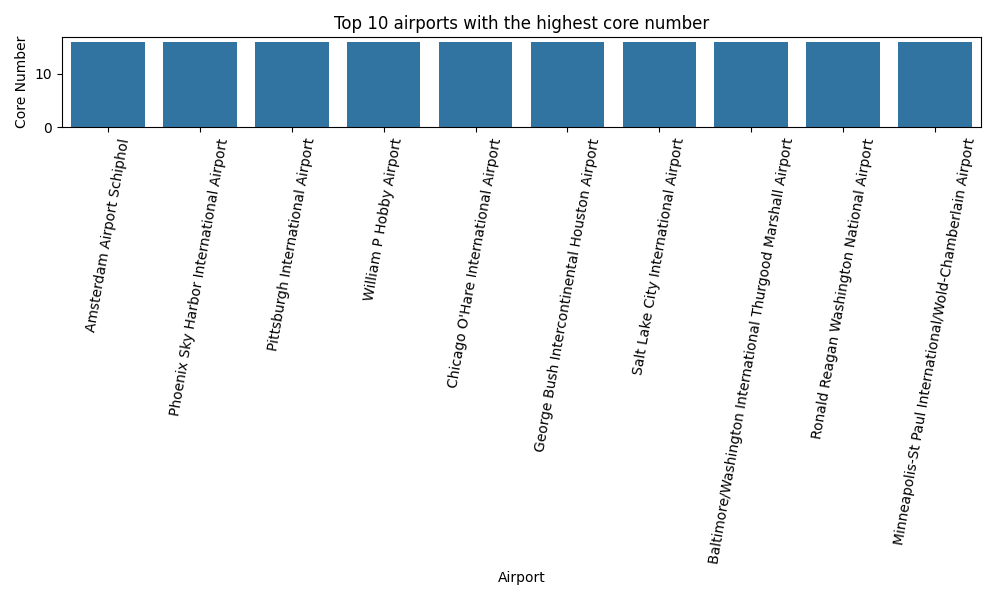
\includegraphics[width=1\linewidth]{img/core_number.png}
\end{minipage}

\begin{minipage}{\textwidth}
    \subsubsection{Eigenvector Centrality}
    {Atlanta's high score (0.52) means it's well-connected to other well-connected airports, making it highly influential in the network. An airport with many connections to small, isolated airports would have a lower eigenvector centrality than one with fewer connections to major hubs.}
    \centering
    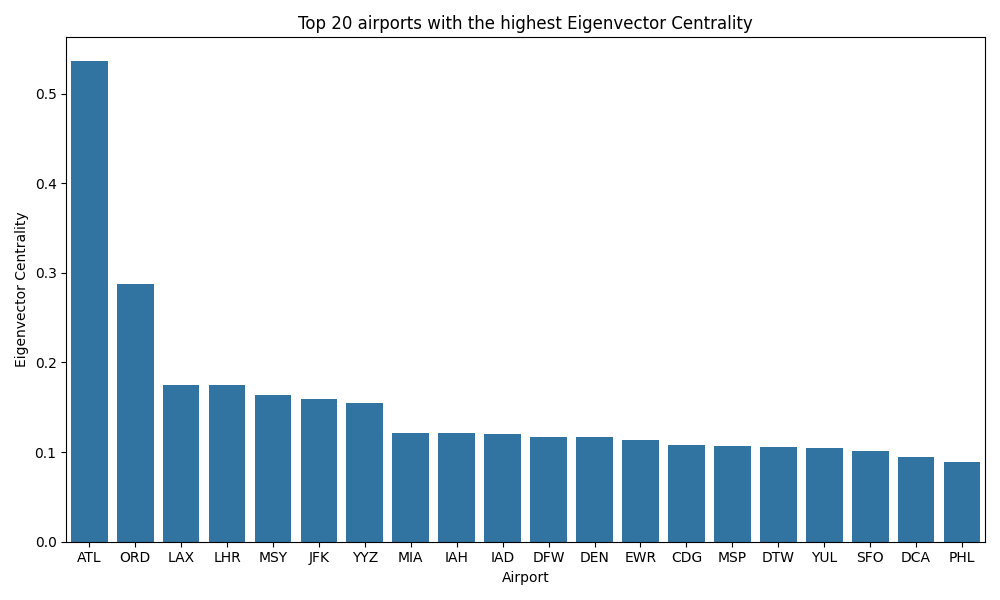
\includegraphics[width=1\linewidth]{img/eigenvector_centrality.png}
\end{minipage}

\begin{minipage}{\textwidth}
    \subsubsection{Pagerank}
    {PageRank scores measure airport importance by considering both quantity and quality of connections.}
    \centering
    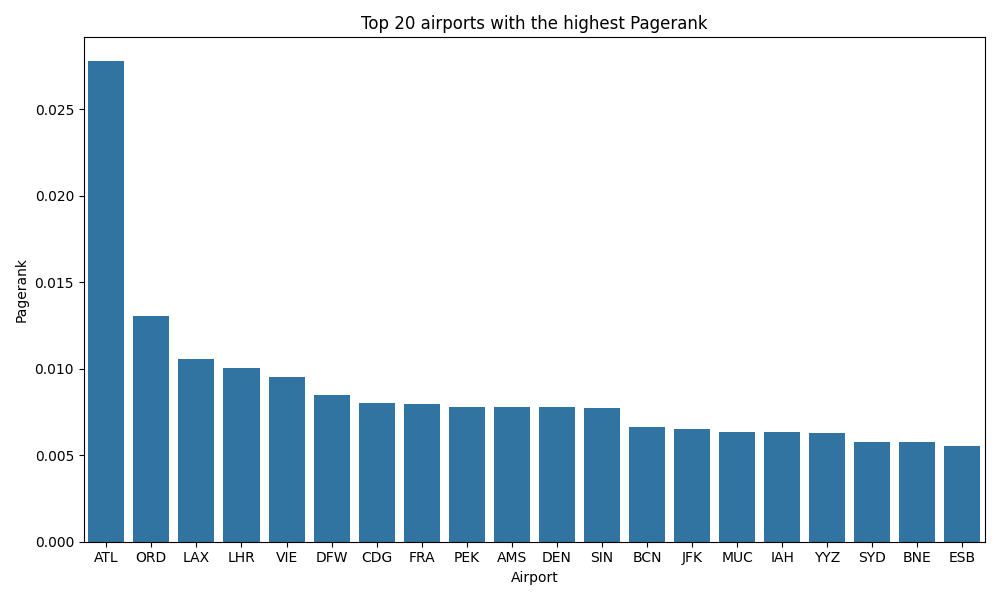
\includegraphics[width=1\linewidth]{img/pagerank.png}
\end{minipage}

\begin{minipage}{\textwidth}
    \subsubsection{Metrics distribution on linear scale}
    {distribution on linear scale of previous metrics}
    \centering
    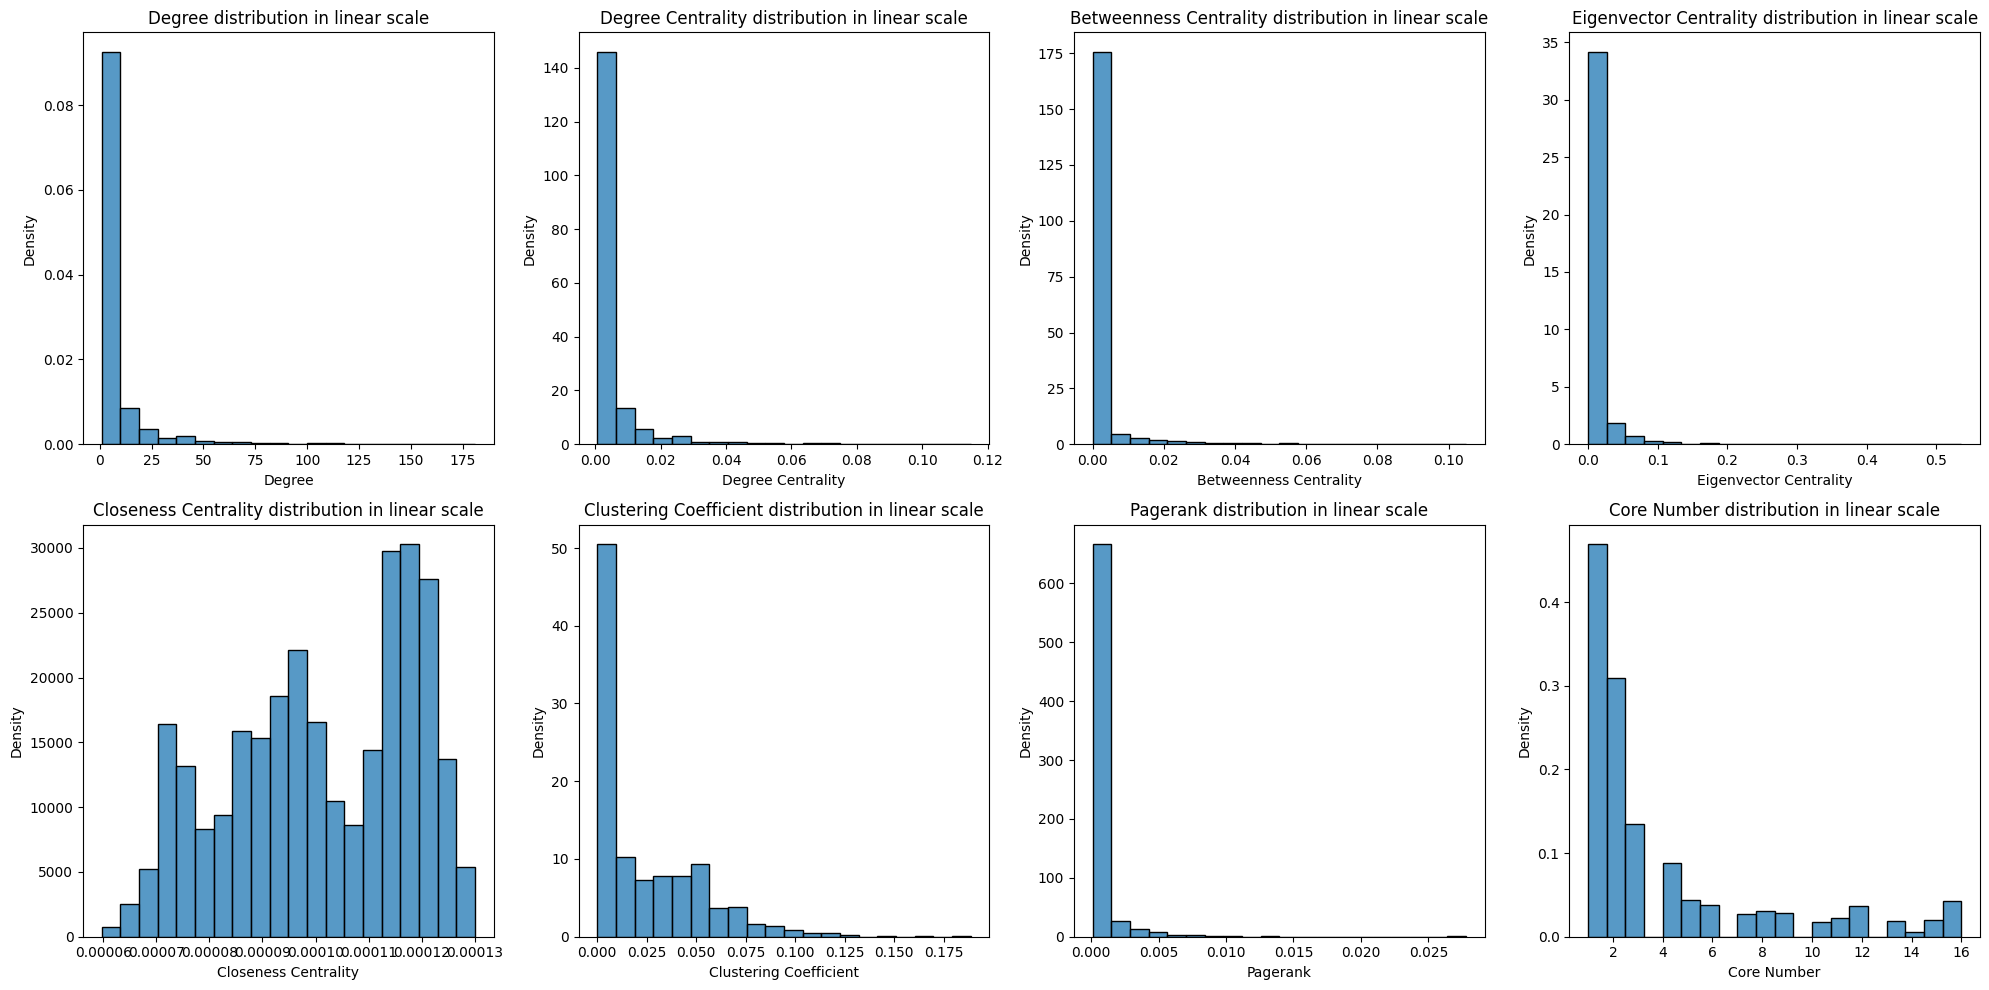
\includegraphics[width=1\linewidth]{img/metrics_output.png}
\end{minipage}

\begin{minipage}{\textwidth}
    \subsubsection{Metrics distribution on log scale}
    {distribution on log scale of previous metrics}
    \centering
    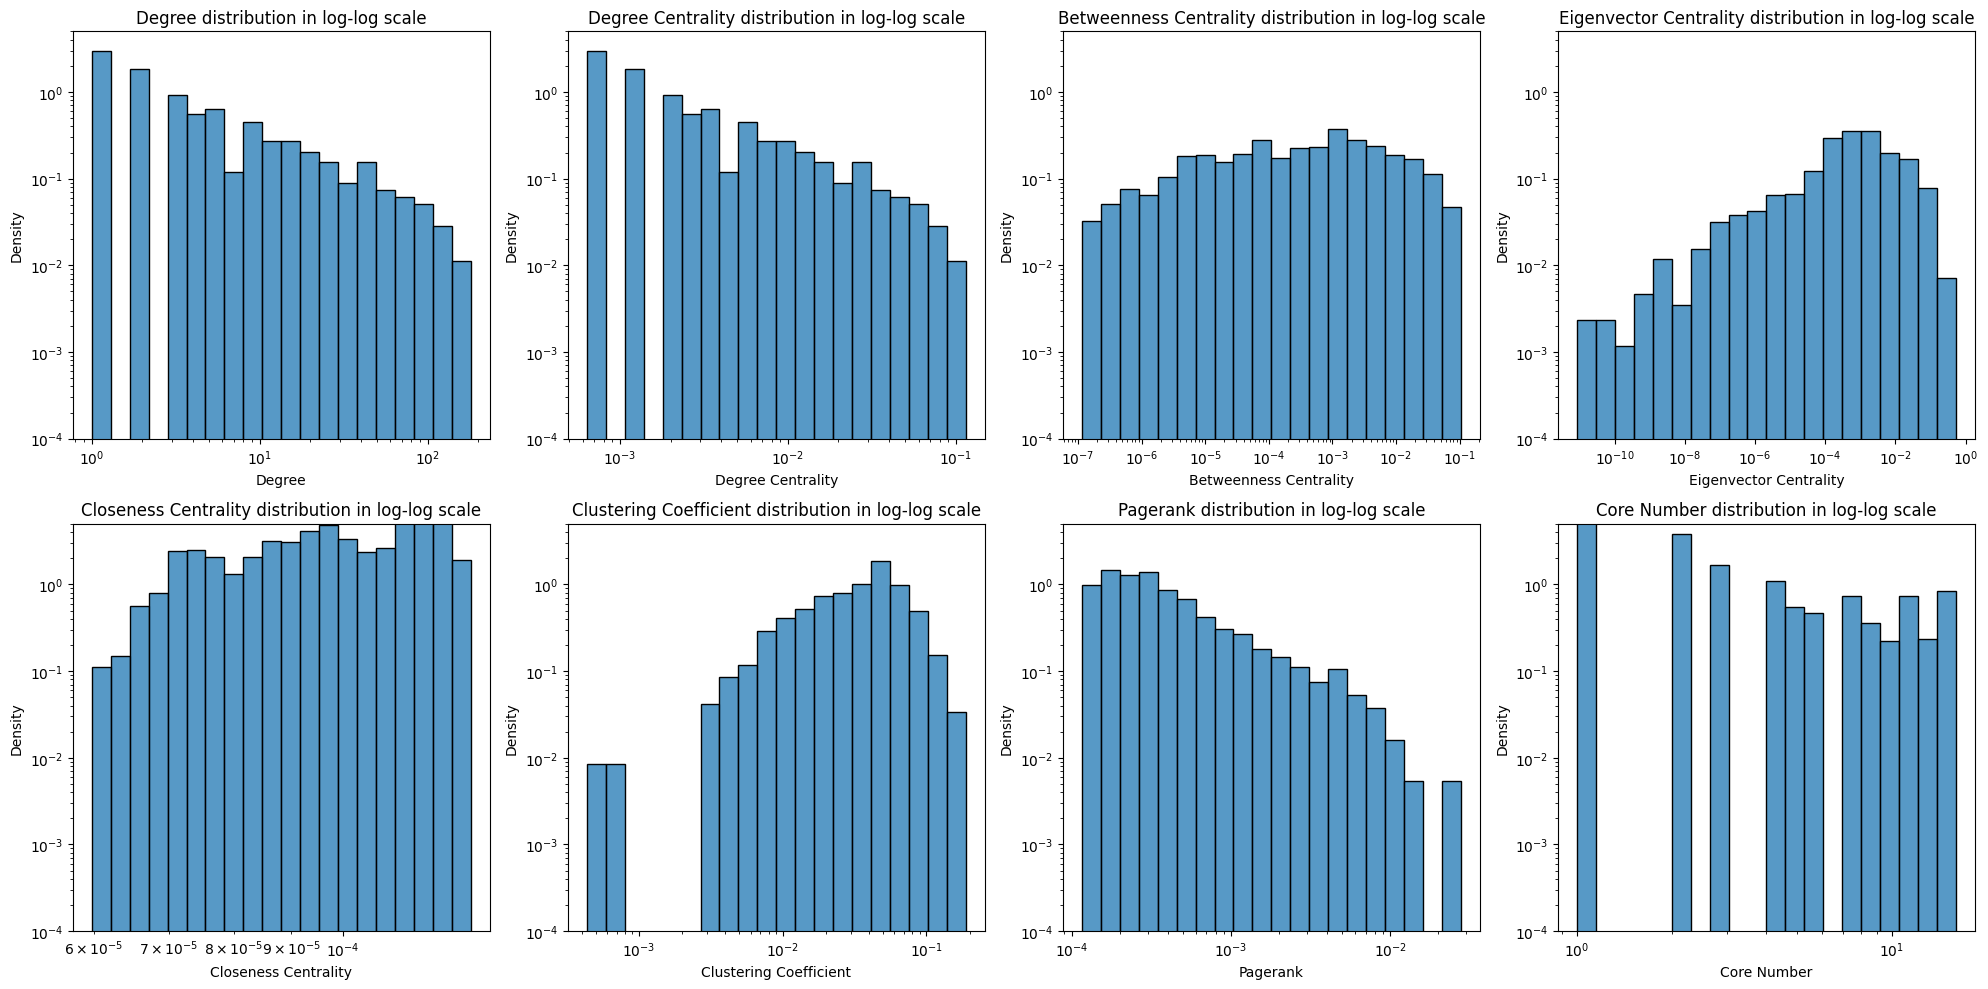
\includegraphics[width=1\linewidth]{img/metrics_logscale_output.png}
\end{minipage}

\begin{minipage}{\textwidth}
    \subsubsection{Density}
    { Is a valuable tool for evaluating how collaborative or fragmented a network is. While intuitively, one might assume that higher density is always better, this is not necessarily the case. Both high and low density have their own advantages and limitations, and the ideal density for any network depends on the goals of the organization. In this case the density is very low. Nodes have fewer redundant connections, potentially leading to more independence and less pressure to constantly engage. However, if the density is too low, members might struggle to collaborate effectively, as communication pathways are fewer, and members may feel isolated.
    }
    \centering
\end{minipage}
\newpage
\begin{minipage}{\textwidth}
    \subsubsection{Clustering}
    {Clustering of airports}
    \centering
    \includegraphics[width=1\linewidth]{img/community_clustering_graph.png}
\end{minipage}

\begin{minipage}{\textwidth}
    \subsubsection{Robustness}
    {The ability of the network to maintain a connection between all (or most) pairs of nodes when challenged. First, our team computed the firts 10 hubs with highest degree value. After that, we've removed them from the network in order to check connectivity. The result was that we lost connectivity after the elimination of the hubs. Follow the fragmentation computation that resulted very low, so, the network is not fragmented. The third step is the computation of compactness. Initially was around 0.25 , but after removing the hubs the network wan't compact anymore.}
\end{minipage}

\begin{minipage}{\textwidth}
    \subsubsection{Centrality Analysis}
    {At the end we proceded with the computation of the betweness centrality. Then we visualized the most influenced airports about the new computation of the metric.}
    \centering
    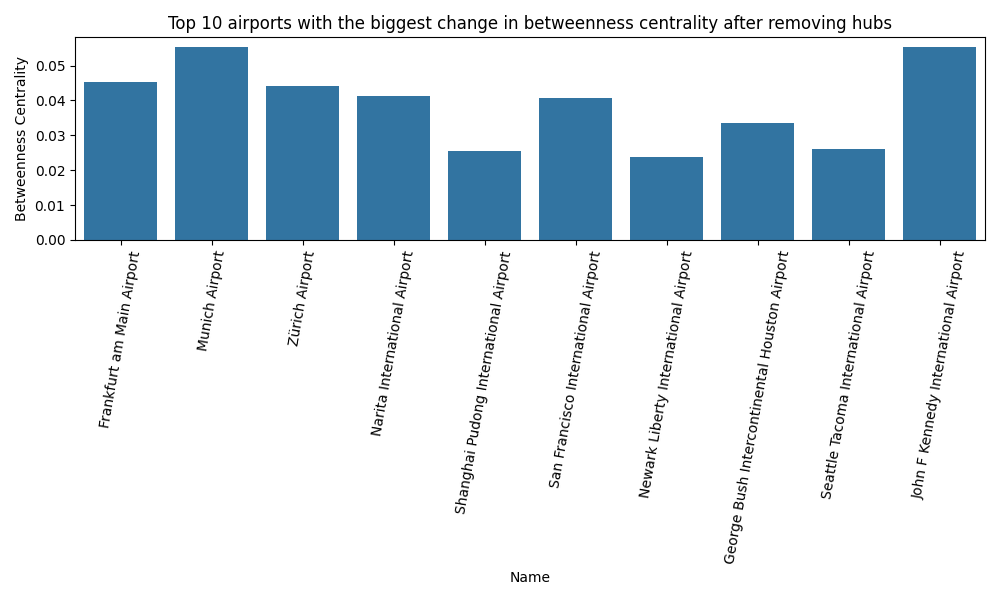
\includegraphics[width=1\linewidth]{img/biggest_changes_betweenness_centrality.png}
\end{minipage}

 
\end{document}